\renewcommand{\thesection}{\Roman{section}}
\section{Limitations}

Even if our method had performed as well on the robot as it did on the test set, there were many limitations to using this approach for object recognition.

First and foremost, the method is limited only to objects which have been observed before. It is designed only to recognize a known object; it does not encode any higher-level characteristics which can then be observed in new objects. The method is also highly dependent on object orientation and size. The neural network needs to have been trained with a grasp of an object in a \emph{particular} orientation in order to be able to recognize that object the next time it is observed in that orientation.

Nor is it invariant to the shape of the hand, since we use raw sensor data rather than extracting a feature vector from local keypoints, as is typical in computer vision. Because of this dependence on hand and finger pose, in order to perform recognition over all the grasp types shown in Section \ref{softarch}, it was necessary to train a \emph{separate} neural network for \emph{each} type, and use the network which corresponds to the current grasp when performing predictions.

We also consider the method likely to break down when number of objects increases. Classification gets significantly harder the more classes you have to decide between (not to mention training becomes much costlier). There is likely to be some point at which splitting hairs between similar classes becomes intractable.

Another drawback is the rather inaccurate tactile sensing. Object shapes do not necessarily show up in the pressure maps of the tactile sensor arrays. Due to the small spatial resolution of the sensor arrays, localization of shape contours is coarse. In addition, the sensors gave repeatedly erroneous feedback (see figure \ref{crazymap}) which made reliability doubtful. Due to the tightness of the grasps, contact surfaces with the fingers are often broad. These particular sensors probably call for a treatment very different from the edge/corner detection of computer vision algorithms, and so we are also unsure about their use in neural network classification.
\begin{figure}[H]
        \hspace{-1.3cm}
         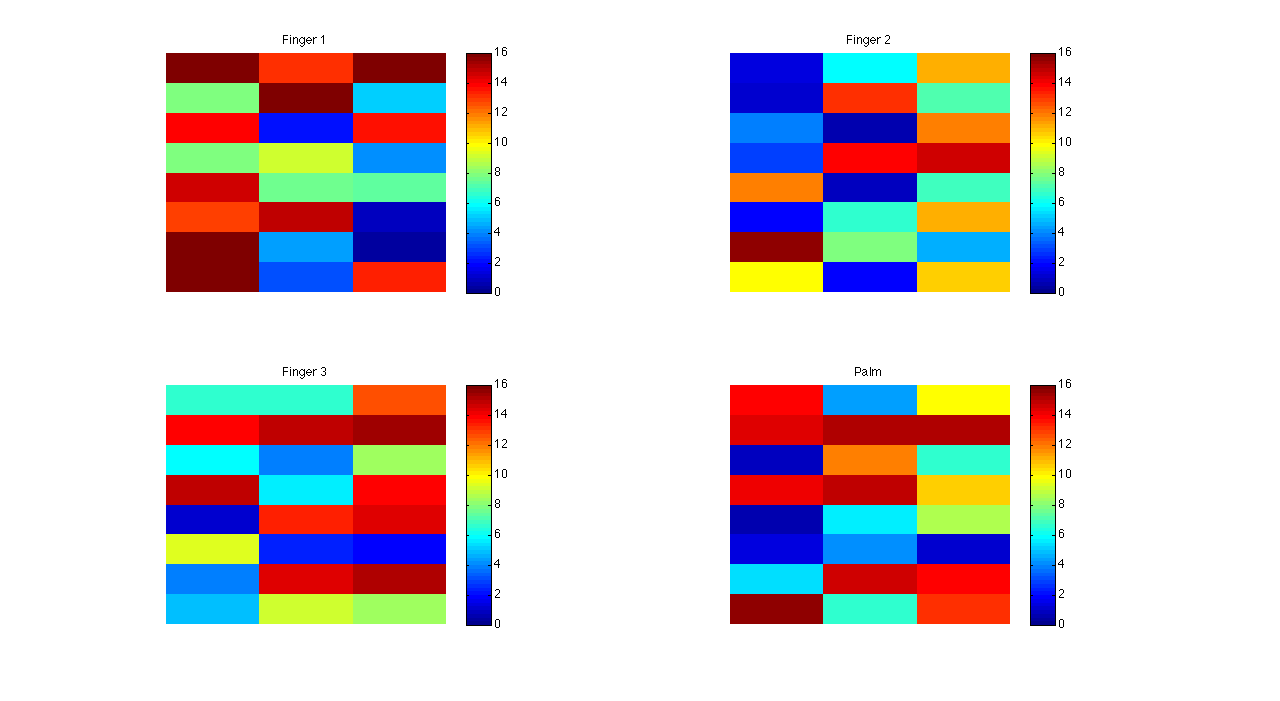
\includegraphics[width=0.6\textwidth]{CrazyPressureM.png}
          \caption{Faulty pressure read out exemplary for top-down prismatic precision grip. Such readout occurred repeatedly for each grasp.}
          \label{crazymap}
\end{figure}